\section{Einleitung}
Sed ut perspiciatis unde omnis iste natus error sit voluptatem accusantium doloremque laudantium, totam rem aperiam, eaque ipsa quae ab illo inventore veritatis et quasi architecto beatae vitae dicta sunt explicabo. Nemo enim ipsam voluptatem quia voluptas sit aspernatur aut odit aut fugit, sed quia consequuntur magni dolores eos qui ratione voluptatem sequi nesciunt. Neque porro quisquam est, qui dolorem ipsum quia dolor sit amet, consectetur, adipisci velit, sed quia non numquam eius modi tempora incidunt ut labore et dolore magnam aliquam quaerat voluptatem.\footcite[Vgl.][]{testOnline} Ut enim ad minima veniam, quis nostrum exercitationem ullam corporis suscipit laboriosam, nisi ut aliquid ex ea commodi consequatur? Quis autem vel eum iure reprehenderit qui in ea voluptate velit esse quam nihil molestiae consequatur, vel illum qui dolorem eum fugiat quo voluptas nulla pariatur?\footcite[Vgl.][S. 83]{testBuch}

\section{Monokulare Tiefenkriterien}
Auch hier was...

\subsection{Erarbeitung der Suchwortliste}
\begin{itemize}
\item monokulare Hinweisreize 
\item monokulares Tiefensehen
\item monokulare Schätzmechanismen
\item monokulare Raumwahrnehmung
\item monoskopisches Tiefensehen
\item monoskopische Schätzmechanismen
\item monoskopische Raumwahrnehmung
\item Monovision
\item monocular depth cues
\end{itemize}


\subsection{Überblick und Ursprung zu den Kriterien}
\marginnote{DD}
Je nach Quelle lassen sich verschiedene monokulare Tiefenkriterien ermitteln. Im wesentlichen handelt es sich bei diesen Unterschieden aber eher um Detailierungsgrade. Je detailierter diese Kriterien unterschieden werden, desto mehr existieren und umgekehrt. Lt. \cite{heidXX} existieren die folgenden monokularen Tiefenkriterien:

\begin{itemize}
\item Verdeckung und Überlappung,
\item Schatten,
\item Vertraute Größe,
\item Relative Helligkeit und perspektivische Unschärfe,
\item Texturdichte-Gradient sowie
\item Relative Höhe / Lage zum Horizont
\end{itemize}

Den oben aufgeführten Kriterien fügt \cite{leyh10} zudem noch die lineare Perspektive hinzu.

\subsection{Verdeckung und Überlappung}
\marginnote{DD}
Das Kriterium Verdeckung und Überlappung lässt den Betrachter Tiefenunterschiede wahrnehmen. Dadurch, dass ein Objekt ein anderes überdeckt kann davon ausgegangen werden, dass wenigstens eine weitere Tiefenebene existiert und dass das verdeckende Objekte näher zum Betrachter ist, als das verdeckte Objekt.\footcite[Vgl.]{heidXX}

\vspace{1em}
\begin{minipage}{\linewidth}
	\centering
	
\includegraphics[width=0.7\linewidth]{images/verdeckung.jpg}
	\captionof{figure}[verdeckung]{Verdeckung}
	\label{fig:verdeckung}
\end{minipage}
\vspace{1em} 

In Abbildung \ref{fig:verdeckung} wird das Kriterium der Verdeckung und Überlappung anhand von zwei Rechtecken dargestellt. Das schwarze Rechteck überlagert das rote Rechteck, wodurch der Eindruck vermittelt wird, dass Ersteres auf der Tiefenebene vor dem Letzterem liegt. Das schwarze Rechteck liegt also näher am Betrachter.

\subsection{Schatten}
\marginnote{DD}
Das Schatten-Kriterium beschreibt, dass ein Betrachter anhand der Länge der Schatten zweier Objekte auf die relative Größe beider Objekte zueinander schließen kann. Ist der Schatten von Objekt A länger als der von Objekt B, ist B größer als A.\footcite[Vgl.][S.43]{Gras16} Voraussetzung dafür ist allerdings, dass beide Schatten unter den selben Bedingungen entstehen.\\

\vspace{1em}
\begin{minipage}{\linewidth}
	\centering
	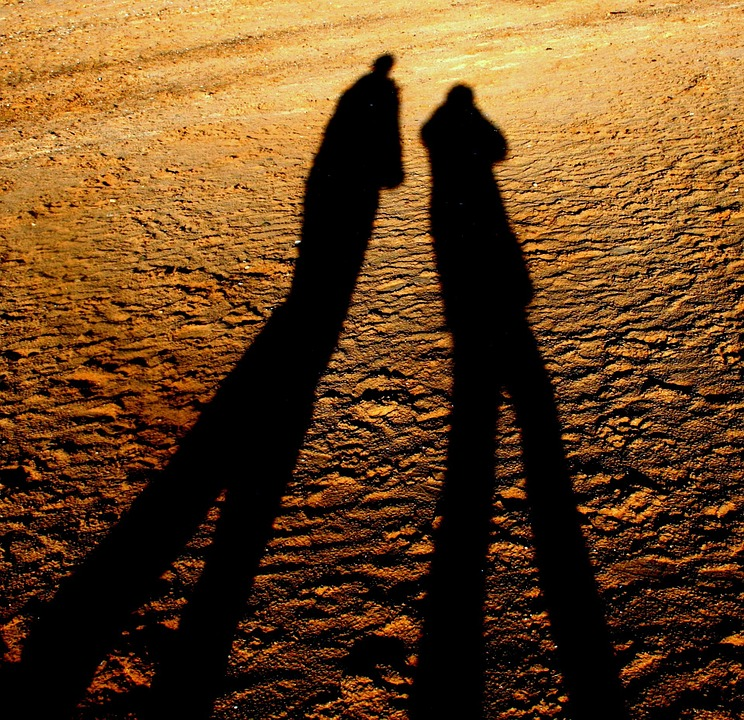
\includegraphics[width=0.7\linewidth]{images/schatten_personen.jpg}
	\captionof{figure}[schatten-relativ]{Schatten zweier Personen (\cite{PixaXX})}
	\label{fig:schatten-relativ}
\end{minipage}
\vspace{1em} 

Abbildung \ref{fig:schatten-relativ} zeigt diesen Sachverhalt. Anhand der Schatten der beiden Personen, lässt sich darauf schließen, dass die rechte Person vermutlich kleiner ist als die linke Person.\\
\\
Außerdem lassen sich durch die Ausrichtung der Schatten  'räumliche Beschaffenheiten' erschließen, wie Abbildung \ref{fig:schatten-raum} zeigt.\footcite[Vgl.]{heidXX} Abbhängig davon, wie die Schatten fallen, ändert sich die Perspektive auf das Objekt.

\vspace{1em}
\begin{minipage}{\linewidth}
	\centering
	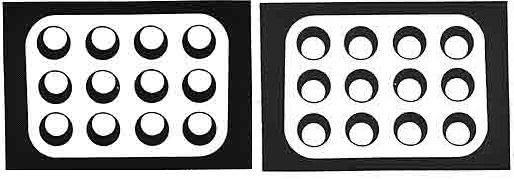
\includegraphics[width=0.7\linewidth]{images/schatten01.jpg}
	\captionof{figure}[schatten-raum]{Räumliche Beschaffenheit (\cite{heidXX})}
	\label{fig:schatten-raum}
\end{minipage}
\vspace{1em} 

\subsection{Vertraute Größe}
\marginnote{DD}
Die vertraute Größe - oder auch relative Größe - erlaubte es, sofern die echte Größe des betrachteten Objekts bekannt ist, die Entfernung zum Objekt zu schätzen. Dies geschieht anhand einer Unterscheidung zwischen der realen Größe und der relativen Größe des Objektes. So können auch gleiche Objekte mit unterschiedlichen relativen Größen als verschieden Weit entfernt erkannt werden.\footcite[Vgl.][S.43]{Ass16}

\vspace{1em}
\begin{minipage}{\linewidth}
	\centering
	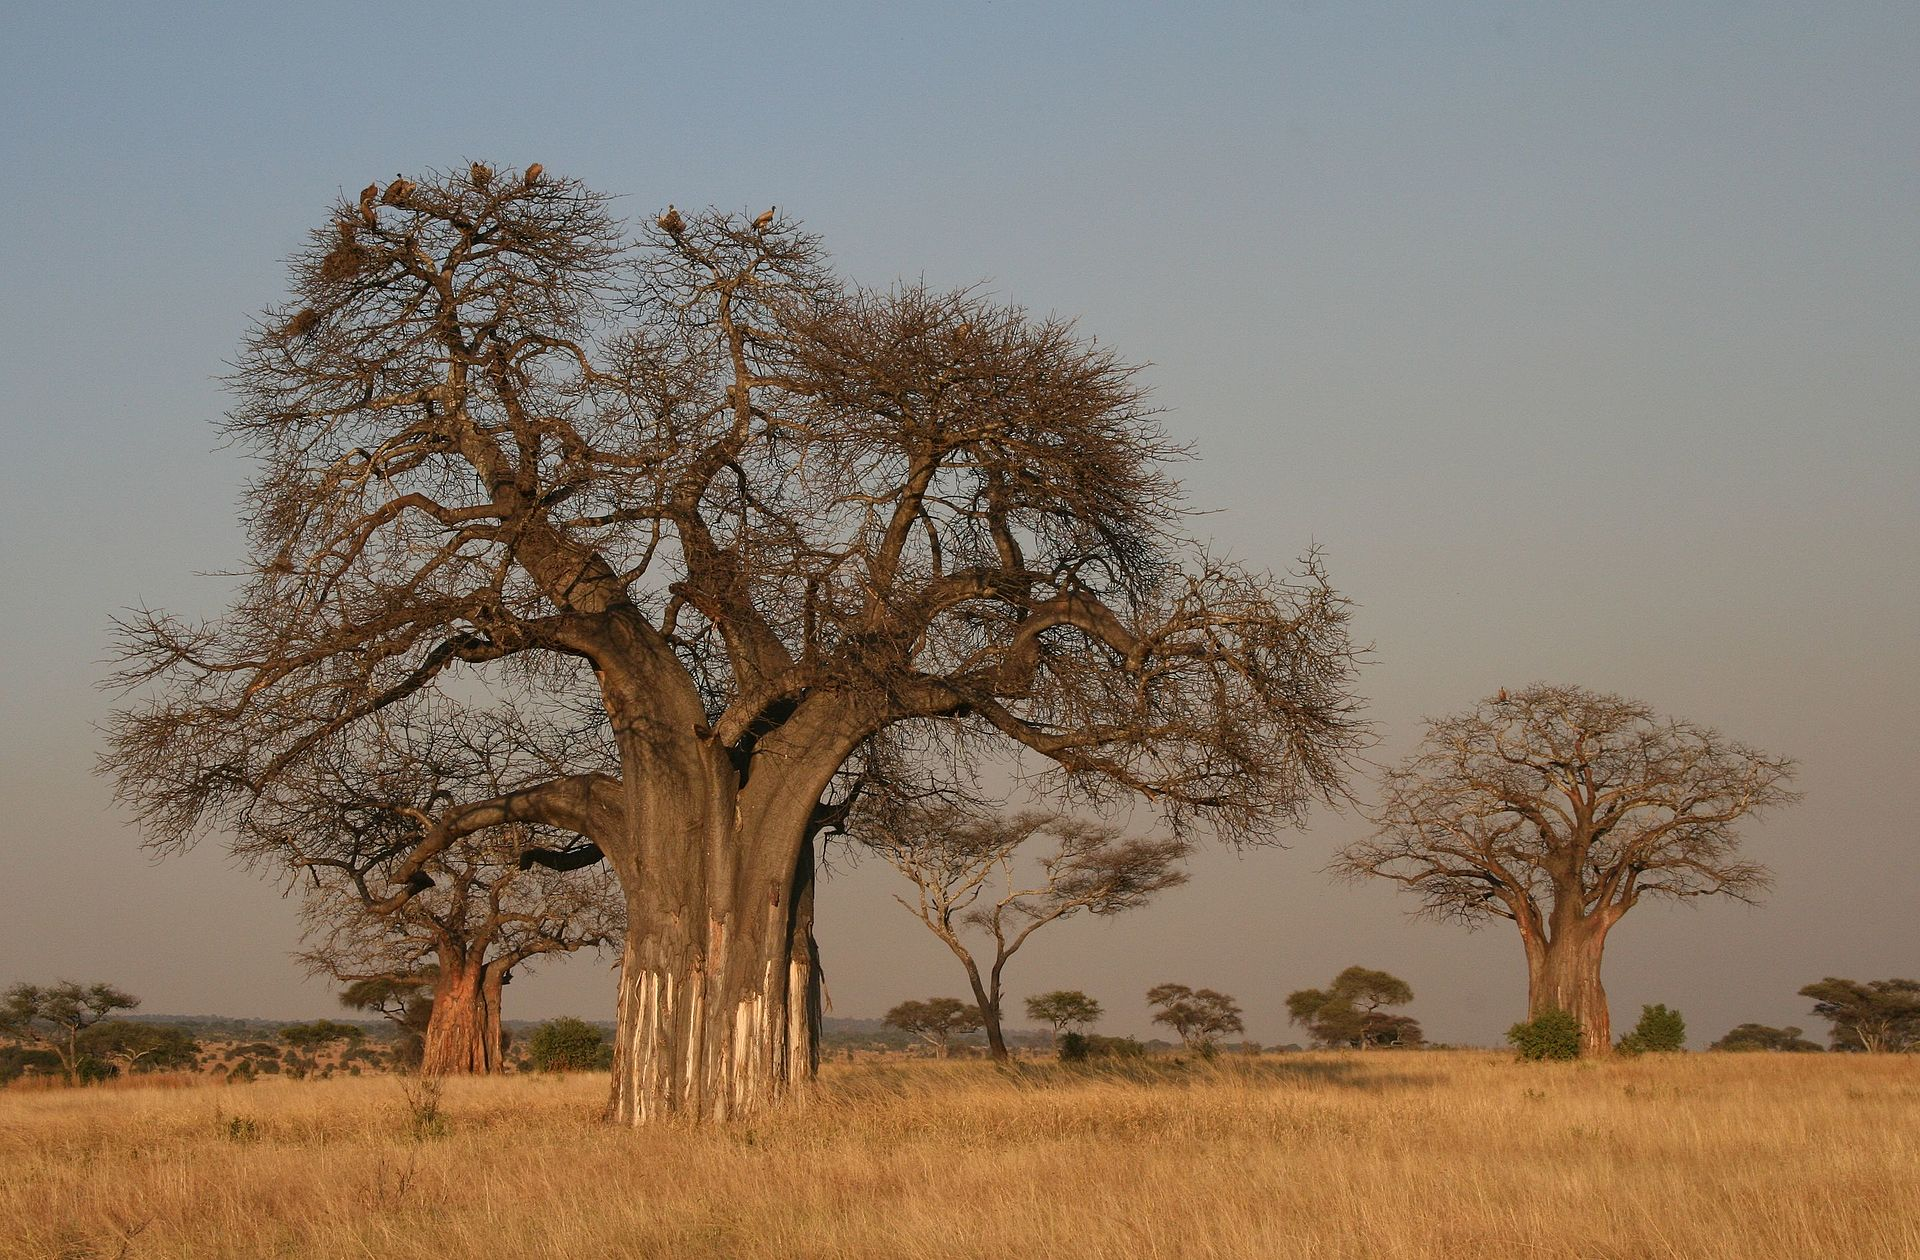
\includegraphics[width=0.7\linewidth]{images/baeume.jpg}
	\captionof{figure}[baeume]{Baumlandschaft (\cite{yokyXX})}
	\label{fig:baeume}
\end{minipage}
\vspace{1em}

Die Abbildung \ref{fig:baeume} verdeutlicht das Kriterium der vertrauten Größe. Es zeigt eine Landschaft mit Bäumen, die unterschiedlich Groß sind. Die kleineren Bäume geraten aufgrund des Kriteriums der vertrauten Größe automatisch in den Hintergrund und die größeren Bäume in den Vordergrund. Demnach erscheinen die größeren Bäume näher zum Betrachter. 

\subsection{Relative Helligkeit und perspektivische Unschärfe}
...

\subsection{Texturdichte-Gradient}
...

\subsection{Lineare Perspektive}
...

\subsection{Relative Höhe / Lage zum Horizont}
...

\subsection{Abgrenzung zu binokularen Tiefenkriterien}
...

\subsection{Anwendungsbereiche im Allgemeinen}
...

\subsection{Reale Beispiele}
...

\section{Konzeption}
...

\section{Umsetzung}
...

\section{Zusammenfassung}
...